%----------------------------------------------------------------------------
\chapter{Követelményspecifikáció}\label{sect:kovspec}
%----------------------------------------------------------------------------

A feladatunk egy családfa-menedzselő alkalmazás megvalósítása Microsoft Silverlight és többrétegű architektúra segítségével. Ennek megfelelően jelen fejezet a \sectref{tervarch} szakaszban a felhasználni kívánt architektúra rövid bemutatását, a \sectref{platform} szakaszban a fejlesztéshez felhasznált platformok, környezetek leírását, a \sectref{funkciok} szakaszban pedig a megvalósítandó funkciók összegzését tartalmazza.

%,,,,,,,,,,,,,,,,,,,,,,,,,,,,,,,,,,,,,,,,,,,,,,,,,,,,,,,,,,,,,,,,,,,,,,,,,,,,
\section{Tervezett architektúra}\label{sect:tervarch}
%,,,,,,,,,,,,,,,,,,,,,,,,,,,,,,,,,,,,,,,,,,,,,,,,,,,,,,,,,,,,,,,,,,,,,,,,,,,,

Az alkalmazás strukturálásához a háromrétegű (multitier) architektúrát\footnote{bővebben: \url{http://en.wikipedia.org/wiki/Multitier\_architecture}} választottuk, amely az \figref{haromreteg} ábrán látható módon épül fel.

\begin{figure}[!ht]
\centering
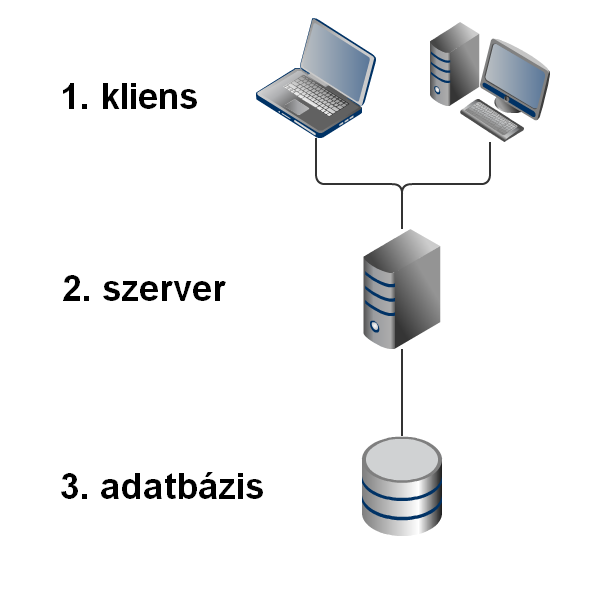
\includegraphics[width=70mm, keepaspectratio]{figures/architektura.png}
\caption{A háromrétegű architektúra.}
\label{fig:haromreteg}
\end{figure}

Az első, \emph{kliens} rétegben a családfák megjelenítését és adminisztrálását végző Silverlight alkalmazás fut -- a felhasználó számítógépén. A második, \emph{webszerver} réteg felelős az alkalmazás webes közzétételéért, valamint itt van lehetőség a működéshez kapcsolódó további statikus vagy dinamikus webes tartalom elhelyezésére. A háttérben, a megjelenítéstől elválasztva, az \emph{adatbázis} rétegben helyezkedik el a családfákat tároló központi adatbázis.

%,,,,,,,,,,,,,,,,,,,,,,,,,,,,,,,,,,,,,,,,,,,,,,,,,,,,,,,,,,,,,,,,,,,,,,,,,,,,
\section{Platform}\label{sect:platform}
%,,,,,,,,,,,,,,,,,,,,,,,,,,,,,,,,,,,,,,,,,,,,,,,,,,,,,,,,,,,,,,,,,,,,,,,,,,,,

Az alkalmazás \emph{kliensrétegében} egy Microsoft Silverlight alkalmazás fut, amely a .NET keretrendszer meglétét igényli a felhasználó számítógépén. Ennek megfelelően a réteg futásához Windows (XP, 2008 Server, Vista, 7), vagy MacOS operációs rendszerre, valamint erre installálva Internet Explorer 7 vagy 8, Mozilla Firefox, Google Chrome, vagy Safari böngészőkre van szükség\footnote{a kompatibilitásról bővebben:  \url{http://en.wikipedia.org/wiki/Microsoft\_Silverlight\#Compatibility}}.

Ezen kívül a Moonlight\footnote{a Moonlight-projekt honlapja: \url{http://www.mono-project.com/Moonlight}} nyílt forráskódú Silverlight-implementációval Linux, OpenBSD, és más Unix-alapú rendszereken is lehetővé válik az alkalmazás futtatása. A dokumentáció írásának pillanatában a Moonlight a Silverlight 2-es verzióját teljes egészében, 3-as verzióját pedig nagyrészt támogatja.

\bigskip

Az alkalmazás \emph{webszerver} rétege dinamikus komponenseket (pl. ASP.NET) nem tartalmaz, ezért bármilyen webszerver-alkalmazás használható a Silverlight-alkalmazás publikálásához. Mi az Apache webszervert választottuk, Linux platformon. Az \emph{adatbázis} réteget egy mySQL adatbázis szolgálja ki, amely szintén Linuxon fut.

%,,,,,,,,,,,,,,,,,,,,,,,,,,,,,,,,,,,,,,,,,,,,,,,,,,,,,,,,,,,,,,,,,,,,,,,,,,,,
\section{Funkciók}\label{sect:funkciok}
%,,,,,,,,,,,,,,,,,,,,,,,,,,,,,,,,,,,,,,,,,,,,,,,,,,,,,,,,,,,,,,,,,,,,,,,,,,,,

A rendszer felhasználói egyéni felhasználói felülettel rendelkeznek, így egyedi azonosításuk szükséges, melyet egy regisztrációs és beléptetési rendszeren keresztül oldunk meg egy felhasználónév-jelszó páros segítségével. A felhasználók központi adminisztrálása (törlés, módosítás) egy egyszerű admin-felületen végezhető.

\bigskip

Egy felhasználó tetszőleges számú családfát hozhat létre, azokat különállóan menedzselheti. A megjelenítés és menedzselés egy összevont felületen történik. Ezen megjelenítési felület három főbb részre osztható:

\begin{enumerate}
 \item kereshető névlista panel
 \item családfa-megjelenítő és -manipuláló felület
  \begin{enumerate}
   \item alapesetben navigálás közben a teljes családfa látszik
   \item a \emph{,,Leszármazott''} nézet bekapcsolásával csak az aktuálisan kiválasztott személy, és azok leszármazottai látszanak
   \item a \emph{,,Származás''} nézet bekapcsolásával csak az aktuális személyt, és őseit jeleníti meg az alkalmazás
  \end{enumerate}
 \item kiválasztott személy részletes élettörténeti adatait megjelenítő panel
\end{enumerate}

A névlista panel segítségével könnyedén és gyorsan eljuthatunk a keresett személyhez. A keresés eredményeképp a fastruktúrájú megjelenítés is a családfa megfelelő részéhez navigál. A hatékony kereséshez egyéb szűrési feltételek is megadhatók (pl. születési év korlát).

A családfa-megjelenítő és -manipuláló felületen lehetőségünk van a családfa skálázható megjelenítésére. Alapvető műveletek a szülő, testvér, gyermek felvétele (esetleg törlése) az aktuálisan kiválasztott (aktív) személyhez. A családfa csomópontjaira kattintva az ott szereplő személy adatait tudjuk módosítani. Továbbá lehetőségünk van az egyes személyekhez képeket rendelni.

Az élettörténeti adatokat részletező panel segítségével felvehetjük és később visszanézhetjük a fontosabb élettörténeti adatokat, például születési hely, lakóhely, munkahely.
